\chapter{QFT en sistemas acelerados y espacio curvo}
%\todo{Corregir numeracion}
C teoría cuántica de campos (QFT) en sistemas acelerados y espacio con curvatura.

\section{Efecto Unruh}

Una propiedad sorprendente de las teorías cuánticas de campos es que el estado de vacío
puede depender del observador.
Concretamente, el efecto Unruh establece que el vacío para un observador inercial,
visto por un observador con aceleración constante corresponde con un estado térmico a temperatura
\begin{equation}
  T_U=\frac{a}{2\pi k_B}.
\end{equation}

En la deducción del efecto Unruh estudiaremos un campo escalar sin masa $\phi(t,z)$ en un espacio de Minkowski
con una dimensión espacial $t$ y una dimensión espacial $z$.  
\footnote{Es posible derivar el efecto Unruh para teorías más generales empleando la integral
  de camino euclídea, véase \cite{Susskind}}
La ecuación que describe el campo es la ecuación de Klein-Gordon
\begin{equation}
  -\pdv[2]{\phi}{t}+\pdv[2]{\phi}{z}=0.
  \label{eq:kg}
\end{equation}

La solución general de esta ecuación de ondas toma la forma
\begin{equation}
  \phi(x,t)=f(t-x)+g(t+x).
\end{equation}

Las funciones $f$ y $g$ representan dos ondas que se mueven a la velocidad de la luz en sentidos
opuestos. 
Hacemos el cambio de variable a coordenadas nulas
\begin{equation}
  U=t-z,   \qquad V=t+z.
\end{equation}

De este modo, la solución general se expresa como
\begin{equation}
  \phi(U,V)=\phi_U(U)+\phi_V(V).
\end{equation}

Nos interesa expandir la solución en términos de ondas armónicas
\begin{gather}
  \phi_\omega^U(U)=\frac{1}{\sqrt{4\pi\omega}} e^{-i\omega U},  \\
  \phi_\omega^V(V)=\frac{1}{\sqrt{4\pi\omega}} e^{-i\omega V}.
\end{gather}

Puesto que la solución $\phi_V$ está desacoplada de $\phi_U$, basta considerar $\phi_U$ ya que
el tratamiento de $\phi_V$ sería análogo.

La expansión del campo en modos es
\begin{equation}
\phi_U(U) = \int_0^\infty d\omega \qty[a_\omega^U \phi_\omega^\phi (U)+a_\omega^{U*} \phi_\omega^\phi (U)^*].
\end{equation}

El proceso de cuantización canónica consiste en reemplazar en valor del campo en cada
punto del espacio-tiempo $\phi(x,t)$, por un operador $\widehat \phi(x,t)$ que satisfará unas
relaciones de conmutación particulares. 
Esto significa que los coeficientes de la expansión de $\phi_U$ pasan a ser los operadores
$\widehat a_\omega^U$ y $\widehat a_\omega^{U\dagger}$ y por tanto
\begin{equation}
  \widehat \phi_U(U) = \int_0^\infty d\omega \qty[\widehat a_\omega^U\phi_\omega^\phi (U)+\widehat a_\omega^{U\dagger} \phi_\omega^\phi (U)^*].
\end{equation}

El operador $\widehat a_\omega^{U\dagger}$ se denomina operador creación, pues veremos que crea 
partículas de frecuencia $\omega$ y $\widehat a_\omega^U$ se conoce como operador destrucción porque
aniquila partículas de frecuencia $\omega$.
Las relaciones de conmutación que cumplen son
\begin{gather}
  [\widehat a_\omega^{U\dagger},\widehat a_{\omega'}^{U\dagger}]=[\widehat a_\omega^U,\widehat a_{\omega'}^U]=0, \\
  [\widehat a_\omega^U,\widehat a_{\omega'}^{U\dagger}]=\delta(\omega-\omega').
\end{gather}

Todavía no hemos especificado el espacio de Hilbert sobre el que actúa el operador del campo, el cual
se denota por $\mathcal H_\phi$. 
El estado del campo queda especificado descrito por un elemento de $\mathcal H_\phi$.
Como en este caso los modos $U$ y $V$ están desacoplados, podemos considerar independientemente el espacio
de Hilbert asociado a cada uno, $\mathcal H_U$ y $\mathcal H_V$.
El espacio de Hilbert del campo es el producto tensorial de ambos $\mathcal H_\phi=\mathcal H_U\otimes \mathcal H_V$.

%Construcción espacio de Fock
La base del espacio $\mathcal H_U$ se puede construir mediante la representación de Fock. 
Para ello, se define el estado de vacío $\ket{0_U}$, como el estado que no contiene ningún tipo
de partícula, por tanto
\begin{equation}
  a^U_\omega \ket{0_U} = 0.
\end{equation}

Donde omitimos el acento circunflejo de los operadores por comodidad.
Luego procedemos a crear estados con $n_i$ partículas de frecuencia $\omega_i$, mediante
aplicación repetida del operador creación $a_{\omega_i}^{U\dagger}$, con la normalización apropiada
\begin{equation}
  \ket{n_{1,\omega_1}, n_{2,\omega_2},\cdots,n_{N,\omega_N}} = \frac{1}{\sqrt{n_1!n_2!\cdots n_N!}}(a_{\omega_1}^{U\dagger})^{n_1}
  (a_{\omega_2}^{U\dagger})^{n_2}\cdots a_{\omega_N}^{U\dagger})^{n_N} \ket{0_U}.
\end{equation}

Los estados construidos son estados propios del operador número de partículas $N_{\omega_i}^U=a_{\omega_i}^{U\dagger}a_{\omega_i}^U$
con valor propio $n_i$.
La base de $\mathcal H_U$ se obtiene juntando los estados con un número arbitrario de partículas
de todas las frecuencias posibles.
%\todo{Definición exacta? La suma directa es no numerable, al tener que considerar todas las frecuencias?}
%Formalmente, $\mathcal H_U$ es la completitud de la suma directa de 
%\todo{Rigor}
%\begin{equation}
%  \mathcal H_U = \overline{\bigoplus  \otimes \ket{n_i}} .
%\end{equation}

%Expansión en otra base. Transformación Bogoliubov. Vacío.
Supongamos que queremos expandir el campo en otra base de modos $u$
\begin{equation}
  \phi_\omega^u(U)=\frac{1}{\sqrt{4\pi\omega}}e^{-i\omega u(U)}, 
\end{equation}

entonces
\begin{equation}
  \phi_U(U) = \int_0^\infty d\omega [a_\omega^u \phi^u_\omega(U) +  a_\omega^{u*} \phi_\omega^u(U)^*].
\end{equation}

Expandiendo la nueva base en términos de la anterior
\begin{equation}
  \phi_\omega^u(U) = \int_0^\infty d\omega'\qty[ \alpha_{\omega\omega'} \phi_{\omega'}^U(U) 
  +\beta_{\omega\omega'} \phi_{\omega'}^U(U)^*].
\end{equation}

Los coeficientes $\alpha_{\omega\omega'}$ y $\beta_{\omega\omega'}$ se denominan coeficientes
de Bogoliubov y vienen dados por
\begin{gather}
  \alpha_{\omega\omega'} = -\frac{1}{2\pi}\sqrt{\frac{\omega'}{\omega}}\int_{-\infty}^\infty dU e^{-i(\omega u(U) -\omega' U)},\\
  \beta_{\omega\omega'} = -\frac{1}{2\pi}\sqrt{\frac{\omega'}{\omega}}\int_{-\infty}^\infty dU e^{-i(\omega u(U) +\omega' U)}.
\end{gather}

Cuantizando la teoría y formando el espacio de Fock, comprobamos que el vacío obtenido mediante
los modos $\phi^U_\omega (U)$, puede contener partículas asociadas a los modos $u$
si el coeficiente $\beta_{\omega\omega'}$ no es nulo
\begin{equation}
  \ev{0_U}{N_\omega^u}=\int_0^\infty d\omega' \abs{\beta_{\omega\omega'}}^2.
\end{equation}

Esto quiere decir que en una teoría cuántica de campos, el vacío depende de la base de modos
que se haya escogido antes de la cuantización.
La ambigüedad se puede resolver escogiendo el vacío que tenga la mínima energía.
En el espacio de Minkowski la energía está bien definida y coincide para todos los observadores
inerciales, al ser invariante de Lorentz.
Sin embargo, en un espacio-tiempo curvo el concepto de energía puede no estar bien definido
y por tanto no hay un estado de vacío privilegiado.

Con el fin de estudiar cuál es el vacío dado por un observador acelerado en un espacio de 
Minkowski, introducimos las coordenadas de Rindler $(\eta,\xi)$ definidas por
\begin{gather}
  t=\frac{1}{a} e^{a\xi} \sinh a\eta ,\\
  z=\frac{1}{a}e^{a\xi} \cosh a\eta,
  \label{eq:rindler}
\end{gather}
donde $\abs{t}<z$ y $a>0$.

Las coordenadas de Rindler solo cubren la región $\abs{t}<z$, denominada cuña derecha de Rindler.
De forma análoga, se puede cubrir la cuña izquierda de Rindler ($\abs{t}<-z$) mediante
las coordenadas $(\tilde \eta, \tilde \xi)$ dadas por
\begin{gather}
  t=-\frac{1}{a} e^{a\tilde \xi} \sinh a\tilde \eta \\
  z=-\frac{1}{a} e^{a\tilde \xi} \cosh a\tilde \eta.
\end{gather}

%Usar imagen libre, centrar
\begin{figure}[htb]
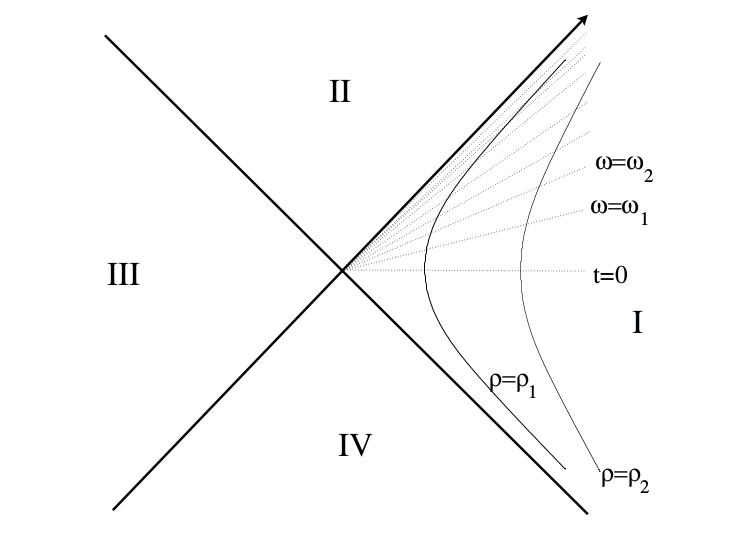
\includegraphics[width=0.8\textwidth]{rindler.png}\hfill
 \caption{Espacio de Minkowski en coordenadas de Rindler (usar imagen libre)
}                   
  \label{fig:rindler}
\end{figure}

Las trayectorias con $\eta=\eta_0$ constante corresponden con observadores que se mueven con
aceleración propia $ae^{-a\xi_0}$.
%\todo{Pq $\xi_0=0$}
El tiempo propio que miden estos observadores es $\tau = e^{a\xi_0}\eta$.
Escogiendo apropiadamente el origen de coordenadas, un observador con aceleración constante
viene dado por $\eta=\tau$ y $\xi=0$.

Fijándonos en el diagrama de Rindler (figura \ref{fig:rindler}),
un observador con aceleración constante moviéndose a la derecha no puede percibir los 
efectos producidos  en III ni influir en II. 
Además, la información que le llegue de II será percibida como proveniente de un tiempo
infinitamente anterior, por lo que la recta $t=z$ define un horizonte de sucesos futuro y 
la recta $t=-z$ un horizonte de sucesos pasado.

Como el observador acelerado hacia la derecha desconoce el estado del campo en la 
cuña izquierda de Rindler, el estado que percibe no es puro, si no mixto.
La descripción de estados mixtos se realiza mediante una matriz de densidad, que al trazar
sobre los estados desconocidos conduce a que el vacío sea un estado térmico.
Con el fin de hacer la deducción explícita, partimos de la ecuación de Klein-Gordon en
coordenadas de Rindler para la cuña derecha
\begin{equation}
  -\pdv[2]{\phi}{\eta}+\pdv[2]{\phi}{\xi} = 0.
  \label{eq:kgr}
\end{equation}

Definiendo las coordenadas nulas de Rindler 
  \begin{align}
    u&=\eta-\xi=-\frac{1}{a}\ln(-aU)\label{eq:coorind} ,\\
    v&=\eta+\xi=\frac{1}{a}\ln(aV), 
  \end{align}

la solución general de \ref{eq:kgr} es $\phi(u,v)=\phi_u(u)+\phi_v(v)$, que se expande en los
modos normales
\begin{equation}
  \begin{aligned}
    \phi^u_\omega(u) &=\frac{1}{\sqrt{4\pi\omega}}e^{-i\omega u},\\
    \phi^u_\omega(v) &=\frac{1}{\sqrt{4\pi\omega}}e^{-i\omega v}.
  \end{aligned}
\end{equation}

Aplicaríamos un tratamiento análogo a la cuña izquierda.

El campo propagándose hacia la derecha en coordenadas de Minkowski se expande como
\begin{equation}
  \begin{aligned}
    \phi_U(U)=&\int_0^\infty \Theta(-U)\qty[a^u_\omega \phi^u_\omega(u(U))+a_\omega^{u*}\phi_\omega^u(u(U))^*] \\
    &+\Theta(U)\qty[a^{\tilde u}_\omega \phi^{\tilde u}_\omega(\tilde u(U))+a_\omega^{\tilde u*}\phi_\omega^{\tilde u}(\tilde u(U))^*].
  \end{aligned}
\end{equation}

Donde $\Theta(U)$ es la función de Heaviside 
\begin{equation}
   \Theta(U)=
  \begin{cases}
    0\qquad \text{si }U<0 \\
    1\qquad \text{si }U>0
  \end{cases}
  .
\end{equation}

El cálculo de los coeficientes de Bogoliubov conduce a 
%\todo{Tal vez separar}
\begin{equation}
  \begin{aligned}
    &\alpha_{\omega,\omega'}^{ u} = -\frac{e^{\frac{\pi\omega}{2 a}}}{2\pi a}\sqrt{\frac{\omega}{\omega'}}\qty(\frac{\omega'}{a})^{-i\omega/a}
    \Gamma(i\omega/a), \quad
    \beta_{\omega,\omega'}^{ u} = \frac{e^{-\frac{\pi\omega}{2 a}}}{2\pi a}\sqrt{\frac{\omega}{\omega'}}\qty(\frac{\omega'}{a})^{-i\omega/a}
    \Gamma(i\omega/a)\\
    &\alpha_{\omega,\omega'}^{\tilde u} = -\frac{e^{\frac{\pi\omega}{2 a}}}{2\pi a}\sqrt{\frac{\omega}{\omega'}}\qty(\frac{\omega'}{a})^{i\omega/a}
    \Gamma(-i\omega/a), \quad
    \beta_{\omega,\omega'}^{\tilde u} = \frac{e^{-\frac{\pi\omega}{2 a}}}{2\pi a}\sqrt{\frac{\omega}{\omega'}}\qty(\frac{\omega'}{a})^{i\omega/a} 
    \Gamma(-i\omega/a)
  \end{aligned}
\end{equation}

Por conveniencia, los modos de Unruh se definen como
\begin{equation}
  \begin{aligned}
    \phi^I_\omega(U)=\Theta(-U)\phi^u_\omega(u(U)) + e^{-\frac{\pi\omega}{a}}\Theta(U)\phi_\omega^{\tilde u}(\tilde u(U))^*,\\
    \phi^{II}_\omega(U)=\Theta(U)\phi^{\tilde u}_\omega(\tilde u(U)) + e^{-\frac{\pi\omega}{a}}\Theta(-U)\phi_\omega^{u}(u(U))^*,
  \end{aligned}
\end{equation}
los cuales están definidos en todo el espacio de Minkowski.

La cuantización de los modos de Unruh conduce a los operadores de destrucción
\begin{equation}
  \begin{aligned}
    a_\omega^I = -2\sinh\frac{\pi\omega}{a}\int_0^\infty d\omega' \beta_{\omega\omega'}^{\tilde u} a_{\omega'}^U,\\
    a_\omega^{II} = -2\sinh\frac{\pi\omega}{a}\int_0^\infty d\omega' \beta_{\omega\omega'}^{u} a_{\omega'}^U.\\
  \end{aligned}
\end{equation}

El vacío de estos modos es el vacío de Minkowski, es decir
\begin{equation}
  a_\omega^I \ket{0_H} = a_\omega^{II}\ket{0_H} = 0.
\end{equation}
 
Para buscar el valor esperado de partículas que observa un observador acelerado
en el vacío de Minkowski, primero calculamos
\begin{equation}
  \ev{a_\omega^{u\dagger}a_\omega^u}{0_H} = \int_0^\infty d\omega'' \beta_{\omega\omega''}^u
  \beta_{\omega'\omega''}^{u*} = \frac{1}{e^{\frac{2\pi\omega}{a}}-1}\delta(\omega-\omega').
\end{equation}

En el límite $\omega'\to\omega$, esta cantidad es el valor esperado de partículas que se
detectarían, pero debido a la delta, se obtiene una divergencia.
El motivo es que calcular el número de partículas en toda la cuña derecha de Rindler, 
implica que hay que considerar un observador acelerado eternamente, lo que requiere infinita
energía.
En una situación real, la delta se transformaría en un valor finito.
Por tanto,
\begin{equation}
  \ev{N_\omega^u}{0_H} \sim \frac{1}{e^{\frac{2\pi\omega}{a}}-1}.
\end{equation}

Este valor esperado se corresponde con un sistema de bosones a temperatura $T=a/(2\pi k_B)$.
Sin embargo, todavía no conocemos la forma exacta del vacío de Minkowski.

En vez de considerar ondas armónicas con frecuencia bien definida, trabajamos con paquetes
de onda con resolución $\Delta \omega$ centrados en $(n+1/2)\Delta \omega$,
\begin{equation}
  \phi_{n\bar n}^u(u)=\frac{1}{\sqrt{\Delta \omega}}\int_{n\Delta\omega}^{(n+1)\Delta \omega}d\omega e^{i\frac{2\pi \bar n n}{\Delta \omega}\omega}
  \phi^u_\omega(u).
\end{equation}

Al cuantizar estos paquetes se introduce para la cuña derecha el operador destrucción $a_{n\bar n}^u$
y en la cuña izquierda $a_{n\bar n}^{\tilde u}$. 
Construyendo los modos de Unruh asociados a paquetes de ondas, se obtiene que
los operadores que los operadores $a_{n\bar n}^I$ y $a_{n\bar n}^{II}$ cumplen
\begin{equation}
  a_{n\bar n}^I\ket{0_U} = a_{n\bar n}^{II} \ket{0_U} = 0.
\end{equation}

De la expresión de $a_{n\bar n}^I$ y $a_{n\bar n}^{II}$ en términos de $a_{n\bar n}^u$ y $a_{n\bar n}^u$, se llega a 
\begin{equation}
  a_{n\bar n}^{u\dagger} a_{n\bar n}^u \ket{0_U} = a_{n\bar n}^{\tilde u\dagger}a_{n\bar n}^{\tilde u} \ket{0_U},
\end{equation}
y por tanto hay el mismo número de partículas asociadas a paquetes de ondas de Rindler en ambas
cuñas.

Teniendo en cuenta que el estado de vacío ha contener el mismo número de partículas en cada cuña,
\begin{equation}
  \ket{0_H} = \prod_{n,\bar n} \qty(\sum_{m=0}^\infty K_{nm} \ket{m_{n\bar n}}_u\otimes \ket{m_{n\bar n}}_{\bar u}).
\end{equation}
\todo{Es $\prod$ un producto tensorial/ suma directa?}

%\begin{equation}
%  K_{n,m+1}=e^{-\frac{\pi n\Delta \omega }{a}}K_{nm}.
%\end{equation}

%\begin{equation}
%  \ket{0_H} = \prod_{n,\bar n} \qty(\sum_{m=0}^\infty e^{-\frac{\pi n\Delta \omega }{a}}K_{nm}\ket{m_{n\bar n}}_u\otimes \ket{m_{n\bar n}}_{\bar u}).
%\end{equation}

Tras calcular los coeficientes $K_{n \bar n}$ y hacer la traza parcial sobre los estados de
la cuña izquierda, obtenemos que la matriz densidad
\begin{equation}
  \rho  \propto \prod_{n,\bar n} \qty(\sum_{m=0}^\infty e^{-2\pi m n\Delta  \omega/a}\ket{m_{n\bar n}}_u \bra{m_{n\bar n}}_u),
\end{equation}
que describe una distribución de Planck a temperatura $T_U=a/(2\pi k_B)$.

%\begin{equation}
%  \ev{0_U}{N^u_{n,\bar n}} =
%\end{equation}


\section{Radiación de Hawking}
La radiación de Hawking consiste en la emisión de partículas por un agujero negro.
Esta radiación sigue una distribución de cuerpo negro a la temperatura de Hawking
\begin{equation}
  T_{haw}= \frac{1}{8\pi k_B G M}.
\end{equation}

Trabajaremos con el caso más sencillo de agujero negro, el agujero negro de Schwarzschild, que
describe una distribución de masa con simetría esférica y estática. La métrica asociada
es 
\begin{equation}
  ds^2= -\qty(1-\frac{2MG}{r})dt^2+\qty(1-\frac{2MG}{r})^{-1}dr^2+r^2d\Omega^2.
\end{equation}

Observamos que en el radio de Schwarzschild $r_s=2MG$, la componente temporal de la 
métrica se anula mientras que la componente radial va a infinito, pero esta singularidad se debe
a la elección particular de coordenadas.
Se denomina horizonte de sucesos a la esfera de radio $r_s$ centrada en $r=0$.
Desde el punto de vista de la relatividad general, la  relevancia del horizonte de sucesos es
que la materia que lo atraviese no podrá salir, sino que se caerá inevitablemente en la singularidad en $r=0$.
Por otro lado, la dilatación temporal de la gravedad  hace que un observador fuera del agujero negro nunca
vea materia atravesar el horizonte, solo la verá moverse arbitrariamente cerca del horizonte.

Es conveniente introducir la coordenada tortuga
\begin{equation}
  r^*=r+2MG\ln\qty(\frac{r}{r_s}-1),
\end{equation}
que toma el valor $r^*=-\infty$ en el horizonte.
La métrica en estas coordenadas es
\begin{equation}
  ds^2= \qty(1-\frac{2MG}{r})[-dt^2+dr^{*2}]+r^2d\Omega^2.
\end{equation}

Si estudiamos un campo escalar no masivo con simetría esférica $\psi(t,r)$, la ecuación de Klein-Gordon
en un espacio de Schwarzschild es
\begin{equation}
  -\pdv[2]{\psi}{t} + \pdv[2]{\psi}{r^{*}} + \frac{2}{r}\qty(1-\frac{r_s}{r}) \pdv{\psi}{r^{*}} = 0.
\end{equation}

Para ver cómo difiere esta ecuación de la ecuación de ondas unidimensional en espacio de Minkowski, hacemos el cambio $\psi=\phi/r$,
\begin{equation}
  -\pdv[2]{\phi}{t} + \pdv[2]{\phi}{r^*} - \frac{r_s}{r^3}\qty(1-\frac{r_s}{r}) \phi= 0.
\end{equation}

Esta ecuación se corresponde con la ecuación de Klein-Gordon que vimos en \ref{eq:kg}, salvo 
por el término de potencial efectivo
\begin{equation}
  V(r) = \frac{r_s}{r^3}\qty(1-\frac{r_s}{r}).
\end{equation}

En una primera aproximación podemos ignorar este potencial, pues su único efecto es distorsionar
la radiación de Hawking emitida (\emph{backscattering}).

Definiendo las coordenadas nulas Eddington-Finkelstein
\begin{equation}
  \begin{aligned}
    u=t-r^*,\\
    v=t+r^*,
  \end{aligned}
\end{equation}
la solución general es
\begin{equation}
  \phi(u,v)=\phi_u(u) + \phi_v(v).
\end{equation}

El campo se descompone en los modos de Boulware
\begin{equation}
  \begin{aligned}
    \phi_\omega^u(u)=\frac{1}{\sqrt{4\pi \omega}}e^{-i\omega u}\\
    \phi_\omega^v(v)=\frac{1}{\sqrt{4\pi \omega}}e^{-i\omega v}.
  \end{aligned}
\end{equation}

El vacío asociado a la cuantización con estos modos se denomina vacío de Boulware y 
corresponde con el vacío que describe un observador en caída libre muy alejado de la fuente
gravitacional.

\subsection{Formación de un agujero negro}

La energía radiada por el agujero negro proviene de la materia que colapsa para formar el agujero negro.
Por tanto, tenemos que describir la formación de un agujero negro y ver cómo varía el estado de vacío
para un observador asintótico.
Suponemos que antes de formarse el agujero negro, la materia ocupa un volumen arbitrariamente grande,
de forma que la métrica fuera del objeto es aproximadamente la métrica de Minkowski y el vacío es el correspondiente
a cuantizar los modos
\begin{equation}
  \begin{gathered}
    \phi_\omega^U (U)=\frac{1}{\sqrt{4\pi\omega}} e^{-i\omega U},\\
    \phi_\omega^V (V)=\frac{1}{\sqrt{4\pi\omega}} e^{-i\omega V},\\
  \end{gathered}
\end{equation}
donde $U=t-r$ y $V=t+r$.

Una vez formado el agujero negro, todo el espacio viene descrito por la métrica de Schwarzschild y
el estado de vacío para observadores inerciales alejados del agujero negro es el vacío de Boulware.
Las partículas que emite el agujero negro y son detectadas por estos observadores se corresponden a los
modos salientes
\begin{equation}
  \phi^u_\omega(u) = \frac{1}{\sqrt{4\pi \omega}}e^{-i\omega u}.
\end{equation}

Tenemos que estudiar cómo se comportan los modos salientes al propagarlos al pasado, cuando todo
el espacio es de Minkowski.
Consideremos los modos que escapan la materia en colapso poco antes de formarse el horizonte.
Cerca del horizonte, si definimos la coordenadas de Kruskal-Szeckeres
\begin{equation}
  \begin{aligned}
    u'&=-4MGe^{-\frac{u}{4MG}},\\
    v'&=4MGe^{-\frac{v}{4MG}},
  \end{aligned}
\end{equation}
los modos salientes son
\begin{equation}
  \phi^{u}_\omega = \frac{1}{\sqrt{4\pi\omega}}e^{i\omega 4MG\ln \abs{\frac{u'}{4MG}}}.
\end{equation}

Vemos que al aproximarse al horizonte, $u'\to 0$, la frecuencia de estos modos tiende a infinito.
Por tanto, podemos despreciar la interacción con la materia en colapso.
La aparición de frecuencias arbitrariamente altas, las cuales deberían ser tratadas mediante
una teoría de gravedad cuántica, se denomina problema transplanckiano.

Como cerca del horizonte la frecuencias son muy altas, los modos se pueden aproximar por rayos (aproximación de la óptica geométrica).
Si definimos $V_H$ de forma que $V=V_H$ es la trayectoria del último rayo que pasa por $r=0$
y logra escapar justo antes de formarse el horizonte, podemos relacionar la coordenada
$u'$ con $V$.
El modo a la distancia nula $u'$ del horizonte se mantendrá en el pasado a la misma distancia de la trayectoria $V=V_H$.
Por tanto,
\begin{equation}
  \phi^{u}_\omega = \frac{1}{\sqrt{4\pi\omega}}e^{i\omega 4MG\ln \abs{A(V_H-V)}}.
\end{equation}

La constante $A$ aparece por la evolución del campo gravitatorio durante el colapso.
Entonces llegamos a la relación entre coordenadas de nulas de Eddington-Finkelstein futuras y de Minkowski pasadas,
que describen la propagación de un rayo que atraviesa el objeto en colapso,
\begin{equation}
  u'=-4MG\ln (A(V_H-V)).
\end{equation}
Esta ecuación es equivalente a la relación entre coordenadas nulas de Rindler y de Minkowski (\ref{eq:coorind}) si identificamos $a=\frac{1}{4MG}$, salvo por las constantes $A$ y $V_H$.
Escogiendo los orígenes de coordenadas de $u$ y $V$ apropiados, la equivalencia se cumple exactamente.
Haciendo un tratamiento análogo al del efecto Unruh, deduciríamos que para tiempo suficientemente tardíos,
los observadores situados en $r\to\infty$ medirían un espectro de radiación correspondiente a un 
cuerpo negro a la temperatura de Hawking,
\begin{equation}
  T_{haw}=\frac{1}{8\pi k_B G M}.
\end{equation}

En el siguiente capítulo, veremos cómo aparece esta misma temperatura al tratar el problema de Hagedorn
cerca de agujeros negros.

\subsection{Deducción alternativa}

La métrica de Schwarzschild, en coordenadas de Rindler, cerca del horizonte se aproxima por 
\begin{equation}
  ds^2= -\frac{\rho^2}{(4GM)^2}dt^2 + d\rho^2 +r^2 d\Omega^2
\end{equation}
donde $\rho = \sqrt{8GM (r-2GM)}$.

Si pasamos a un tiempo imaginario, $t\to \tau=it$, la métrica se convierte en
\begin{equation}
  ds^2= \frac{\rho^2}{(4GM)^2}d\tau^2 + d\rho^2 +r^2 d\Omega^2.
\end{equation}

Esta métrica se corresponde al espacio euclídeo descrito en coordenadas polares.
Para que la métrica no sea singular, el tiempo euclídeo debe tener periodo $\beta=8\pi G M$.

